\section{Introduction}
\label{sec:intro}



{\color{red} TODO: Some Security Background}



\begin{figure}[t!]
\begin{center}
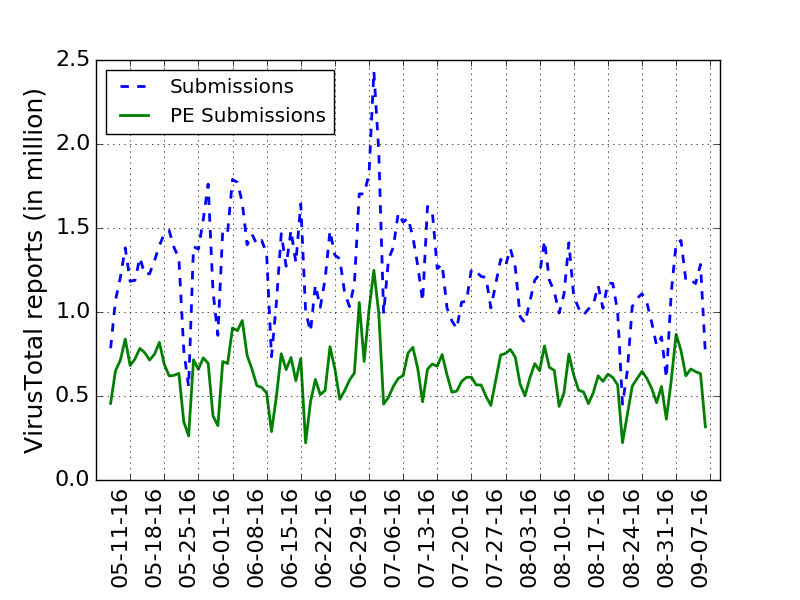
\includegraphics[width=2in]{figure/Submissions}
\caption{The number of files and PE files.
%{\footnotesize{
(The number of suspicious files and the number of PE files submitted to VirusTotal from 05/07/2016 to 09/06/2016.)
%}
}
\label{fig:subnum}
\end{center}
%\vspace{-0.25in}
\end{figure}


VirusTotal provides a valuable resource to study and 
understand real-world malwares and anti-virus engines. 

First, there are huge amount of suspicious files submitted to VirusTotal. 
As shown in Figure~\ref{fig:subnum}, 
there are around 40 million submissions on VirusTotal each month. 
These submissions cover a large variety of file types, and 
are conducted by a large variety of VirusTotal users from all over the world. 
This amount of diverse data on VirusTotal serves as a good representation of malwares in the real world.  

Second, for around all submissions, 
VirusTotal applies no less than 50 state-of-the-art anti-virus engines to analyze them. 
VirusTotal keeps detailed detection results, and provide access to these results. 
Analyzing historical detection results can help capture how anti-virus engines evolve over time. 

Third, VirusTotal provides rich metadata for each submission. 
Besides detection results from different engines, 
VirusTotal also provides file type information, which can help categorize malwares, 
source ID (country), which can help understand popularity of malwares, 
ssdeep digest string, by using which we can calculate code similarity without accessing binary executable, and so on. 


{\color{red} TODO: Existing works on VirusTotal}

In this paper, we collect 4-month (05/07/2016 - 09/06/2016) metadata from VirusTotal,
and conduct a thorough study on these data. 
Following previous works~\cite{SongAPsys2016} on study VirusTotal,
we focus our study on PE files, 
which occupy more than half of VirusTotal’s submissions.
Our study can improve the understanding of malwares and anti-virus engines in the real world, 
and provide implications for future works to apply machine learning to malware detection. 
Our study is mainly conducted in three aspects: 


First, we study the correlation between submissions’ metadata and their detection rates. 
Given a submission, 
we calculate its detection rate as the percentage of engines labeling the submission as malware. 
Higher detection rate indicates a more malicious submission viewed by engines.  
We study correlation between detection rate and source ids’ reputation, submission history, file size and source country. 
Our studying results can help understand which types of malwares are more malicious, 
help security experts invest their limited manual efforts, 
and help anti-virus vendors identify possible false positives and false negatives in their products.  


Second, we study influence among different antivirus vendors. 
One malware could be submitted to VirusTotal more than once. 
For each submission, VirusTotal will apply a bunch of anti-virus engines to analyze it.
We have observed that for some malwares, some anti-virus engines fail to detect them at the first time, while they catch up in later analysis. 
We assume that there is influence among different anti-virus vendors, 
and some anti-virus vendors will follow detection results from other vendors. 
We apply models from web social network area to characterize 
which vendors are more likely to be influenced by others, 
and predict whether detection results from some vendors may change in the future.  

Third, we build a malware detector and classifier based on ssdeep similarity. 
SSDeep is a fuzzy hash algorithm, which takes a file as input and generates a fuzzy hash string as information digest. 
The similarity between fuzzy hashes is an estimation of similarity between the two original files. 
Fuzzy hash for each submission is also calculated and provided by VirusTotal. 
We explore how to use similarity between SSDeep fuzzy hash as 
kernel function to conduct malware classification and malware detection. 